%\newcommand{\wsname}{SemEval-2014}
%\newcommand{\submissionpage}{\url{http://alt.qcri.org/semeval2014/index.php?id=cfp}}
%\newcommand{\filename}{semeval2014}
%\newcommand{\contact}{pnakov qf.org.qa}

\title{SemEval-2014 Task 5: L2 Writing Assistant}
\chapter{SemEval-2014 Task 5: L2 Writing Assistant}

\label{chap:semeval2014task5}

%\author{Maarten van Gompel, Iris Hendrickx,\\ {\bf Antal van den Bosch}\\
%  Centre for Language Studies, \\
%Radboud University Nijmegen,\\
%  The Netherlands\\
%  {\tt proycon@anaproy.nl}, \\
%  {\tt i.hendrickx@let.ru.nl}, \\
%  {\tt a.vandenbosch@let.ru.nl} \\\And
%  Els Lefever and V\'{e}ronique Hoste\\
%  LT3, \\ Language and Translation Technology Team, \\
%Ghent University, \\ Belgium \\ {\tt els.lefever@ugent.be}, \\ {\tt veronique.hoste@ugent.be} }

In this chapter, we present a new cross-lingual task for SemEval concerning the
translation of L1 fragments in an L2 context. The task is derived from the
ideas and findings explored in Chapter~\ref{chap:colibritapilot}.  The task is
at the boundary of Cross-Lingual Word Sense Disambiguation and Machine
Translation and finds application in the field of computer-assisted
translation, particularly in the context of second language learning.
Translating L1 fragments in an L2 context allows language learners when writing
in a target language (L2) to fall back to their native language (L1) whenever
they are uncertain of the right word or phrase.

\textsc{This chapter is based on: }
\bibentry{SEMEVAL2014TASK5}

%footnote without marker
\newcommand\blfootnote[1]{%
\begingroup
\renewcommand\thefootnote{}\footnote{#1}%
\addtocounter{footnote}{-1}%
\endgroup
}

\section{Introduction} %rewritten

\blfootnote{This chapter is licensed under a Creative Commons Attribution 4.0 International Licence: http://creativecommons.org/licenses/by/4.0/}

We present a new cross-lingual and application-oriented task for SemEval that
is situated in the area where Word Sense Disambiguation and Machine Translation
meet. Finding the proper translation of a word or phrase in a given context is
much like the problem of disambiguating between multiple senses.

In this task participants are asked to build a translation/writing assistance
system that translates specifically marked L1 fragments in an L2 context to
their proper L2 translation. This type of translation can be applied in writing
assistance systems for language learners in which users write in a target
language, but are allowed to occasionally back off to their native L1 when they
are uncertain of the proper lexical or grammatical form in L2. The task
concerns the NLP back-end rather than any user interface.

Full-on machine translation typically concerns the translation of complete
sentences or texts from L1 to L2. This task, in contrast, focuses on smaller
fragments, side-tracking the problem of full word reordering.


We focus on the following language combinations of L1 and L2 pairs:
\emph{English-German}, \emph{English-Spanish}, \emph{French-English} and
\emph{Dutch-English}. Task participants could participate for all language
pairs or any subset thereof.


\section{Task Description}

We frame the task in the context of second language learning, yielding a
specific practical application.

Participants build a \emph{translation assistance system}\/ rather than a full
machine translation system. The L1 expression, a word or phrase, is translated
by the system to L2, given the L2 context already present, including right-side
context if available. The aim here, as in all translation, is to carry the
semantics of the L1 fragment over to L2 and find the most suitable L2
expression given the already present L2 context.

Other than a limit on length (6 words), we do not pose explicit constraints on
the kinds of L1 fragments allowed. The number of L1 fragments is limited to one
fragment per sentence.

The task addresses both a core problem of WSD, with cross-lingual context, and
a sub-problem of Phrase-based Statistical Machine Translation; that of finding
the most suitable translation of a word or phrase.  In MT this would be
modelled by the translation model. In our task the full complexity of
full-sentential translation is bypassed, putting the emphasis on the semantic
aspect of translation. Our task has specific practical applications and a
specific intended audience, namely intermediate and advanced second language
learners, whom one generally wants to encourage to use their target language as
much as possible, but who may often feel the need to fall back to their native
language.

Currently, language learners are forced to fall back to a bilingual dictionary
when in doubt. Such dictionaries do not take the L2 context into account and
are generally more constrained to single words or short expressions. The
proposed application would allow more flexible context-dependent lookups as
writing progresses. The task tests how effectively participating systems
accomplish this.

The following examples illustrate the task for the four language pairs we
offer:


\begin{itemize}
  \item
    Input (L1=English,L2=Spanish): \emph{“Todo ello, \textbf{ in accordance}  con los principios que siempre hemos apoyado.”} \\
    Desired output: \emph{“Todo ello,  \textbf{de conformidad} con los principios que siempre hemos apoyado.”}
  \item
    Input (L1-English, L2=German): \emph{“Das, was wir heute machen, \textbf{is essentially} ein Ärgernis.”} \\
    Desired output: \emph{“Das, was wir heute machen, \textbf{ist im Grunde genommen} ein Ärgernis.”}
  \item
    Input (L1=French,L2=English): \emph{“I \textbf{rentre à la maison} because
    I am tired.”} \\
    Desired output: \emph{“I \textbf{return home} because I am tired.”}
  \item
    Input (L1=Dutch, L2=English): \emph{“Workers are facing a massive \textbf{aanval
    op} their employment and social rights.”} \\
    Desired output: \emph{“Workers are facing a massive \textbf{attack on}
    their employment and social rights.”}
\end{itemize}


The task can be related to the two tasks that were offered in previous years of
SemEval and already introduced in Chapter~\ref{clwsd}: Lexical Substitution
\citep{CLLS} and most notably Cross-lingual Word Sense Disambiguation
\citep{Lefever2013}.

When comparing our task to the Cross-Lingual Word-Sense Disambiguation task,
one notable difference is the fact that our task concerns not just words, but
also phrases. Another essential difference is the nature of the context; our
context is in L2 instead of L1. Unlike the Cross-Lingual Word Sense
Disambiguation task, we do not constrain the L1 words or phrases that may be
used for translation, except for a maximum length which we set to 6 tokens,
whereas Lefever and Hoste (2013) only tested a select number of nouns. Our task
emphasizes a correct meaning-preserving choice of words in which translations
have to fit in the L2 context. There is thus a clear morphosyntactic aspect to
the task, although less prominent than in full machine translation, as the
remainder of the sentence, already in L2, does not need to be changed.  In the
Cross-Lingual Word Sense Disambiguation tasks, the translations/senses were
lemmatised. We deliberately chose a different path that allows for the
envisioned application to function directly as a translation assistance system.

Chapter~\ref{chap:colibritapilot} described a pilot study conducted to test the
feasibility of the proposed translation system. It shows that L2 context
information can be a useful cue in translation of L1 fragments to L2, improving
over a non-context-informed baseline.


\section{Data}
\label{sec:data}

We did not provide training data for this task, as we did not want to bias
participating systems by favouring a particular sort of material and
methodology. Moreover, it would be a prohibitively large task to manually
collect enough training data of the task itself. Participants were therefore
free to use any suitable training material such as parallel corpora, wordnets,
or bilingual lexica.

Trial and test data has been collected for the task, both delivered in a simple
XML format that explicitly marks the fragments. System output of participants
adheres to the same format. The trial set, released early on in the task, was
used by participants to develop and tune their systems on. The test set
corresponds to the final data released for the evaluation period; the final
evaluation was conducted on this data.

The trial data was constructed in an automated fashion in the way described in
Chapter~\ref{chap:colibritapilot}. In summary, first a phrase-translation table is
constructed from a parallel corpus. We used the Europarl parallel corpus
\citep{EUROPARL} and the Moses tools \citep{MOSES}, which in turn makes use of
GIZA$++$ \citep{GIZA}. Only strong phrase pairs (exceeding a set threshold) were
retained and weaker ones were pruned. This phrase-translation table was then
used to create input sentences in which the L2 fragments are swapped for their
L1 counterparts, effectively mimicking a fall-back to L1 in an L2 context. The
full L2 sentence acts as reference sentence. Finally, to ensure all fragments
are correct and sensible, a manual selection from this automatically generated
corpus constituted the final trial set.

In the pilot study in Chapter~\ref{chap:colibritapilot}, such a data set, even
without the manual selection stage, proved adequate to demonstrate the
feasibility of translating L1 fragments in an L2 context. One can, however,
rightfully argue whether such data is sufficiently representative for the task
and whether it would adequately cover instances where L2 language learners
might experience difficulties and be inclined to fall back to L1.  We therefore
created a more representative test set for the task.

The actual test set conforms to much more stringent constraints and was
composed entirely by hand from a wide variety of written sources. Amongst these
sources are study books and grammar books for language learners, short
bilingual on-line stories aimed at language learners, gap-exercises and cloze
tests, and contemporary written resources such as newspapers, novels, and
Wikipedia. We aimed for actual learner corpora, but finding suitable learner
corpora with sufficient data proved hard. For German we could use the the
Merlin corpus \citep{Merlin}. In example (a) we see a real example of a fragment
in a fallback language in an L2 context from the Merlin corpus.

\begin{examples}
\footnotesize
\item[(a)] \textbf{Input:} Das Klima hier ist \textbf{Tropical} und wir haben fast keinen Winter\\
 \textbf{Reference:} Das Klima hier ist \textbf{tropisch} und wir haben fast keinen Winter.
\end{examples}


For various sources bilingual data was available. For the ones that were
monolingual (L2) we resorted to manual translation. To ensure our translations
were correct, these were later independently verified, and where necessary
corrected by native speakers.

A large portion of the test set comes from off-line resources because we wanted
to make sure that a substantial portion of the test set could not be found
verbatim on-line. This was done to prevent systems from solving the actual
problem by just attempting to just look up the sources through the available
context information.

Note that in general we aimed for the European varieties of the different
languages. However, for English we did add the US spelling variants as
alternatives.

% Here is an example from the English-French test set that shows how the XML format looks like and how alternative translations are marked with the tag <alt>.
%\begin{examples}
%\label{ex2}
%\item[(a)] <ref>Keegan passes to Smith , who runs straight at the <f id="1">central defence<alt>central defense</alt><alt>key defence</alt><alt>key defense</alt></f>  and shoots , and Gomez pushes it over the bar for a corner .</ref>
%\end{example}
A complete list of all sources used in establishing the test set is available on our website\footnote{https://github.com/proycon/semeval2014task5}.

%Iris> zouden we niet beter verwijzen naar de originele Semeval pagina? Maarten> Nee, die is nu overbodig, alles staat op github

We created a trial set and test set/gold standard of 500 sentence pairs per
language pair. Due to the detection of some errors at a later stage, some of
which were caused by the tokenisation process, we were forced to remove some
sentences from the test set and found ourselves slightly below our aim for some
of the language pairs. The test set was delivered in both
tokenised\footnote{Using ucto, available at https://github.com/proycon/ucto}
and untokenised form. The trial set was delivered only in tokenised form.
Evaluation was conducted against the tokenised version, but our evaluation
script was designed to be as lenient as possible regarding differences in
tokenisation. We explicitly took cases into account where participant's
tokenisers split contractions (such as Spanish ``del'' to ``de'' $+$ ``el''),
whereas our tokeniser did not.

For a given input fragment, it may well be possible that there are multiple
correct translations possible. In establishing our test set, we therefore paid
special attention to adding alternatives. To ensure no alternatives were
missed, all participant output was aggregated in one set, effectively
anonymising the systems, and valid but previously missed alternatives were
added to the gold standard.


\section{Evaluation}
\label{sec:semeval2014task5evaluation}

Several metrics are available for automatic evaluation. First, we measure the
absolute accuracy $a = c/n$, where $c$ is the number of fragment translations
from the system output that precisely match the corresponding fragments in the
reference translation, and $n$ is the total number of translatable fragments,
including those for which no translation was found. We also introduce a
word-based accuracy, which unlike the absolute accuracy gives some credits to
mismatches that show partial overlap with the reference translation.  It
assigns a score according to the longest consecutive matching substring between
output fragment and reference fragment and is computed as follows:

\begin{equation}
wac = \frac{|longestsubmatch(output,reference)|}{max(|output|,|reference|)}
\end{equation}

The system with the highest word-based accuracy wins the competition. All
matching is case-sensitive.

Systems may decide not to translate fragments if they cannot find a suitable
translation. A recall metric simply measures the number of fragments for which
the system generated a translation, regardless of whether that translation is
correct or not, as a proportion of the total number of fragments.

In addition to these task-specific metrics, standard MT metrics such as BLEU,
NIST, METEOR and error rates such as WER, PER and TER, are included in the
evaluation script as well. Scores such as BLEU will generally be high ($>
0.95$) when computed on the full sentence, as a large portion of the sentence
is already translated and only a specific fragment remains to be evaluated.
Nevertheless, these generic metrics are proven in our pilot study to follow the
same trend as the more task-specific evaluation metrics, and will be omitted in
the result section for brevity.

It regularly occurs that multiple translations are possible. As stated, in the
creation of the test set we have taken this into account by explicitly encoding
valid alternatives. A match with any alternative in the reference counts as a
valid match. For word accuracy, the highest word accuracy amongst all possible
alternatives in the reference is taken. Likewise, participant system output may
contain multiple alternatives as well, as we allowed two different types of
runs, following the example of the Cross-Lingual Lexical Substitution and
Cross-Lingual Word Sense Disambiguation tasks:

\begin{itemize}
     \item \textbf{Best} - The system may only output one, its best, translation;
     \item \textbf{Out of Five} - The system may output up to five alternatives, effectively allowing 5 guesses. Only the best match is counted. This metric does \emph{not} count how many of the five are valid.
\end{itemize}

Participants could submit up to three runs per language pair and evaluation type.

\section{Participants}

Six teams submitted systems, three of which participated for all language pairs. In alphabetic order, these are:

\begin{enumerate}
\item \textbf{CNRC} - Cyril Goutte, Michel Simard, Marine Carpuat - National Research Council Canada -- \emph{All language pairs}
\item \textbf{IUCL} - Alex Rudnick, Liu Can, Levi King, Sandra Kübler, Markus Dickinson - Indiana University (US) -- \emph{all language pairs}
\item \textbf{UEdin} - Eva Hasler - University of Edinburgh (UK) -- \emph{all language pairs except English-German}
\item \textbf{UNAL} - Sergio Jiménez, Emilio Silva - Universidad Nacional de Colombia -- \emph{English-Spanish}
\item \textbf{Sensible} - Liling Tan - Universität des Saarlandes (Germany) and Nanyang Technological University (Singapore) -- \emph{all language pairs}
\item \textbf{TeamZ} - Anubhav Gupta - Université de Franche-Comté (France) -- \emph{English-Spanish, English-German}
\end{enumerate}

Participants implemented distinct methodologies and implementations. One
obvious avenue of tackling the problem is through standard Statistical Machine
Translation (SMT). The CNRC team takes a pure SMT approach with few
modifications. They employ their own Portage decoder and directly send an L1
fragment in an L2 context, corresponding to a partial translation hypothesis
with only one fragment left to decode, to their decoder \citep{CNRC}. The UEdin
team applies a similar method using the Moses decoder, marking the L2 context
so that the decoder leaves this context as is. In addition they add a context
similarity feature for every phrase pair in the phrase translation table, which
expresses topical similarity with the test context. In order to properly
decode, the phrase table is filtered per test sentence \citep{UEDIN}. The IUCL
and UNAL teams do make use of the information from word alignments or phrase
translation tables, but do not use a standard SMT decoder. The IUCL system
combines various information sources in a log-linear model: phrase table, L2
Language Model, Multilingual Dictionary, and a dependency-based collocation
model, although this latter source was not finished in time for the system
submission \citep{IUCL}. The UNAL system extracts syntactic features as a means
to relate L1 fragments with L2 context to their L2 fragment translations, and
uses memory-based classifiers to achieve this \citep{UNAL}. The two systems on
the lower end of the result spectrum use different techniques altogether. The
Sensible team approaches the problem by attempting to emulate the manual
post-editing process human translators employ to correct MT output
\citep{SENSIBLE},
%maar hoe doen ze het dan?
whereas TeamZ relies on Wiktionary as the sole source \citep{TEAMZ}.


\section{Results}

The results of the six participating teams can be viewed in consensed form in
Table \ref{tab:results}. This table shows the highest word accuracy achieved by
the participants, in which multiple system runs have been aggregated. A ranking
can quickly be distilled from this, as the best score is marked in bold. The
system by the University of Edinburgh emerges as the clear winner of the task.
The full results of the various system runs by the six participants are shown
in Tables~\ref{tab:fullresults1} and \ref{tab:fullresults2}, two pages down,
all three aforementioned evaluation metrics are reported there and the systems
are sorted by word accuracy per language pair and evaluation type.


For the lowest-ranking participants, the score is negatively impacted by the low recall; their systems could not find translations for a large number of fragments.

Figures~\ref{fig:graphs} (next page) and \ref{fig:graphs2} (last page) show the
results for the \emph{best} evaluation type for each system run. Three bars are
shown; from left to right these represent \emph{accuracy} (blue),
\emph{word-accuracy} (green) and \emph{recall} (red). Graphs for
\emph{out-of-five} evaluation were omitted for brevity, but tend to follow the
same trend with scores that are somewhat higher. These scores can be viewed on
the result website at \url{http://github.com/proycon/semeval2014task5/}. The
result website also holds the system output and evaluation scripts with which
all graphs and tables can be reproduced.

We observe that the best scoring team in the task (UEdin), as well as the CNRC
team, both employ standard Statistical Machine Translation and achieve high
results. From this we can conclude that standard SMT techniques are suitable
for this task. Teams IUCL and UNAL achieve similarly good results, building on
word and phrase alignment data as does SMT, yet not using a traditional SMT
decoder. TeamZ and Sensible, the two systems ranked lowest do not rely on any
techniques from SMT. To what extent the context-informed measures of the
various participants are effective can not be judged from this comparison, but
can only be assessed in comparison to their own baselines. For this we refer to
the system papers of the participants.


\begin{table}[bt]
{\footnotesize
\noindent\makebox[\textwidth][c]{%
\begin{tabular}{llll}
\hline
System                & Acc & W.Acc. & Recall    \\ \hline
\multicolumn{4}{|c|}{\textbf{English-Spanish (best)}} \\
\hline
UEdin-run2          & 0.755    & 0.827         & 1.0                 \\
UEdin-run1          & 0.753    & 0.827         & 1.0                 \\
UEdin-run3          & 0.745    & 0.82          & 1.0                 \\
UNAL-run2           & 0.733    & 0.809         & 0.994\\
UNAL-run1           & 0.721    & 0.794         & 0.994\\
CNRC-run1           & 0.667    & 0.745         & 1.0                 \\
CNRC-run2           & 0.651    & 0.735         & 1.0                 \\
IUCL-run1           & 0.633    & 0.72          & 1.0                 \\
IUCL-run2           & 0.633    & 0.72          & 1.0                 \\
Sensible-wtmxlingyu & 0.239    & 0.351         & 0.819\\
TeamZ-run1          & 0.223    & 0.333         & 0.751\\
Sensible-wtm        & 0.145    & 0.175         & 0.470 \\
Sensible-wtmxling   & 0.141    & 0.171         & 0.470 \\
\hline
\multicolumn{4}{|c|}{\textbf{English-Spanish (out-of-five)}} \\
\hline
UEdin-run3          & 0.928    & 0.949         & 1.0                 \\
UEdin-run1          & 0.924    & 0.946         & 1.0                 \\
UEdin-run2          & 0.92     & 0.944         & 1.0                 \\
CNRC-run1           & 0.843    & 0.887         & 1.0                 \\
CNRC-run2           & 0.837    & 0.884         & 1.0                 \\
UNAL-run1           & 0.823    & 0.88          & 0.994\\
IUCL-run1           & 0.781    & 0.847         & 1.0                 \\
IUCL-run2           & 0.781    & 0.847         & 1.0                 \\
Sensible-wtmxlingyu & 0.263    & 0.416         & 0.819\\
TeamZ-run1          & 0.277    & 0.386         & 0.751\\
Sensible-wtm        & 0.173    & 0.231         & 0.470 \\
Sensible-wtmxling   & 0.169    & 0.228         & 0.470 \\
\hline
\multicolumn{4}{|c|}{\textbf{English-German (best)}} \\
\hline
 IUCL-run2           & 0.665    & 0.722         & 1.0                 \\
 CNRC-run1           & 0.657    & 0.717         & 1.0                 \\
CNRC-run2           & 0.645    & 0.702         & 1.0                 \\
TeamZ-run1          & 0.218    & 0.293         & 0.852 \\
IUCL-run1           & 0.198    & 0.252         & 1.0                 \\
Sensible-wtmxlingyu & 0.162    & 0.233         & 0.878\\
Sensible-wtm        & 0.16     & 0.184         & 0.647\\
Sensible-wtmxling   & 0.152    & 0.178         & 0.647\\
\hline
\multicolumn{4}{|c|}{\textbf{English-German (out-of-five)}} \\
\hline
CNRC-run1           & 0.834    & 0.868         & 1.0                 \\
CNRC-run2           & 0.828    & 0.865         & 1.0                 \\
IUCL-run2           & 0.806    & 0.857         & 1.0                 \\
TeamZ-run1          & 0.307    & 0.385         & 0.852\\
IUCL-run1           & 0.228    & 0.317         & 1.0                 \\
Sensible-wtmxlingyu & 0.18     & 0.306         & 0.878\\
Sensible-wtm        & 0.182    & 0.256         & 0.647\\
Sensible-wtmxling   & 0.174    & 0.25          & 0.647\\
\hline
\end{tabular}}
\caption{Full results for English-Spanish and English-German.}
\label{tab:fullresults1}
}
\end{table}



\begin{table}[tb]
{\small
\noindent\makebox[\textwidth][c]{%
\begin{tabular}{llll}
\hline
System                & Acc & W.Acc. & Recall    \\ \hline
\multicolumn{4}{|c|}{\textbf{French-English (best)}} \\
\hline
UEdin-run1          & 0.733    & 0.824         & 1.0                 \\
UEdin-run2          & 0.731    & 0.821         & 1.0                 \\
UEdin-run3          & 0.723    & 0.816         & 1.0                 \\
CNRC-run1           & 0.556    & 0.694         & 1.0                 \\
CNRC-run2           & 0.533    & 0.686         & 1.0                 \\
IUCL-run1           & 0.545    & 0.682         & 1.0                 \\
IUCL-run2           & 0.545    & 0.682         & 1.0                 \\
Sensible-wtmxlingyu & 0.081    & 0.116         & 0.321  \\
Sensible-wtm        & 0.055    & 0.067         & 0.210  \\
Sensible-wtmxling   & 0.055    & 0.067         & 0.210  \\
\hline
\multicolumn{4}{|c|}{\textbf{French-English (out-of-five)}} \\
\hline
UEdin-run2          & 0.909    & 0.939         & 1.0                 \\
UEdin-run1          & 0.905    & 0.938         & 1.0                 \\
UEdin-run3          & 0.907    & 0.937         & 1.0                 \\
CNRC-run1           & 0.739    & 0.839         & 1.0                 \\
CNRC-run2           & 0.731    & 0.834         & 1.0                 \\
IUCL-run1           & 0.691    & 0.8           & 1.0                 \\
IUCL-run2           & 0.691    & 0.8           & 1.0                 \\
Sensible-wtmxlingyu & 0.085    & 0.14          & 0.321  \\
Sensible-wtmxling   & 0.061    & 0.09          & 0.210  \\
Sensible-wtm        & 0.061    & 0.089         & 0.210  \\
\hline
\multicolumn{4}{|c|}{\textbf{Dutch-English (best)}} \\
\hline
UEdin-run1          & 0.575    & 0.692         & 1.0                 \\
UEdin-run2          & 0.567    & 0.688         & 1.0                 \\
UEdin-run3          & 0.565    & 0.688         & 1.0                 \\
IUCL-run1           & 0.544    & 0.679         & 1.0                 \\
IUCL-run2           & 0.544    & 0.679         & 1.0                 \\
CNRC-run1           & 0.45     & 0.61          & 1.0                 \\
CNRC-run2           & 0.444    & 0.609         & 1.0                 \\
Sensible-wtmxlingyu & 0.115    & 0.152         & 0.335 \\
Sensible-wtm        & 0.092    & 0.099         & 0.214 \\
Sensible-wtmxling   & 0.088    & 0.095         & 0.214 \\
\hline
\multicolumn{4}{|c|}{\textbf{Dutch-English (out-of-five)}} \\
\hline
UEdin-run1          & 0.733    & 0.811         & 1.0                 \\
UEdin-run3          & 0.727    & 0.808         & 1.0                 \\
UEdin-run2          & 0.725    & 0.808         & 1.0                 \\
IUCL-run1           & 0.634    & 0.753         & 1.0                 \\
IUCL-run2           & 0.634    & 0.753         & 1.0                 \\
CNRC-run1           & 0.606    & 0.723         & 1.0                 \\
CNRC-run2           & 0.602    & 0.721         & 1.0                 \\
Sensible-wtmxlingyu & 0.123    & 0.171         & 0.335 \\
Sensible-wtm        & 0.099    & 0.115         & 0.214 \\
Sensible-wtmxling   & 0.096    & 0.112         & 0.214 \\ \hline
\end{tabular}}
}
\caption{Full results for French-English and Dutch-English.}
\label{tab:fullresults2}
\end{table}


\begin{figure*}[p]
\noindent\makebox[\textwidth][c]{%
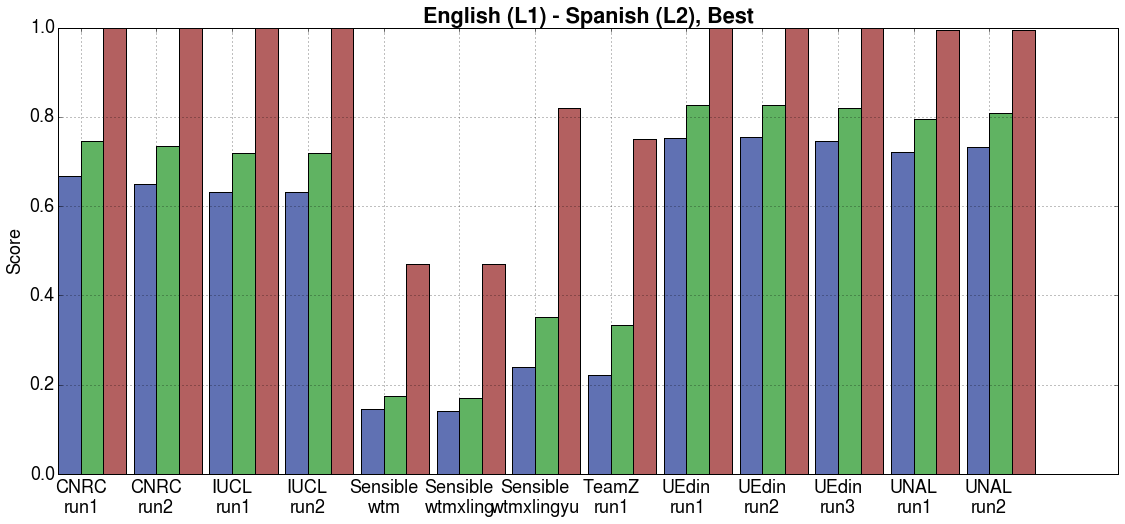
\includegraphics[width=16cm]{en-es-best-2.png}}
\noindent\makebox[\textwidth][c]{%
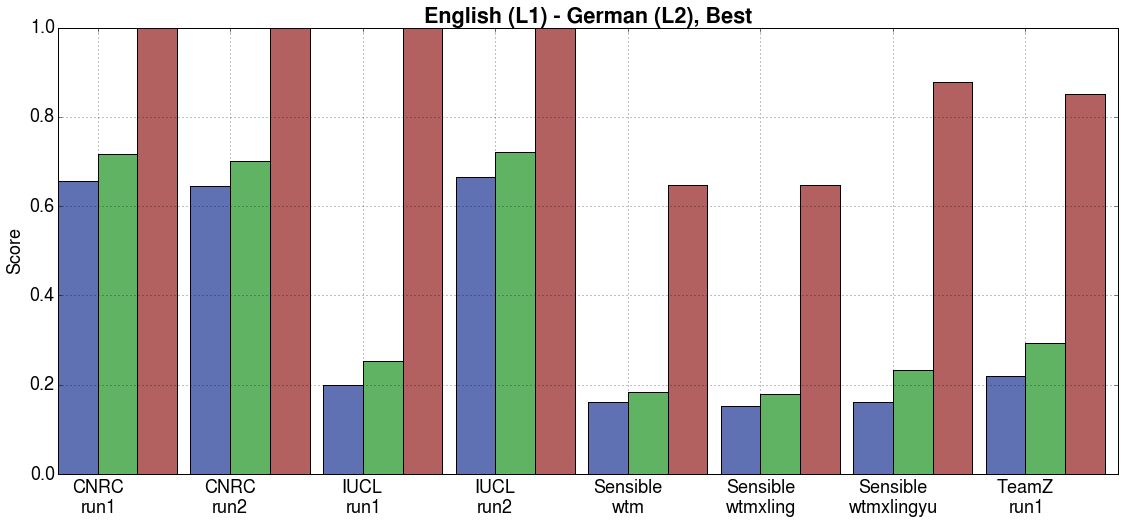
\includegraphics[width=16cm]{en-de-best-2.png}}
\noindent\makebox[\textwidth][c]{%
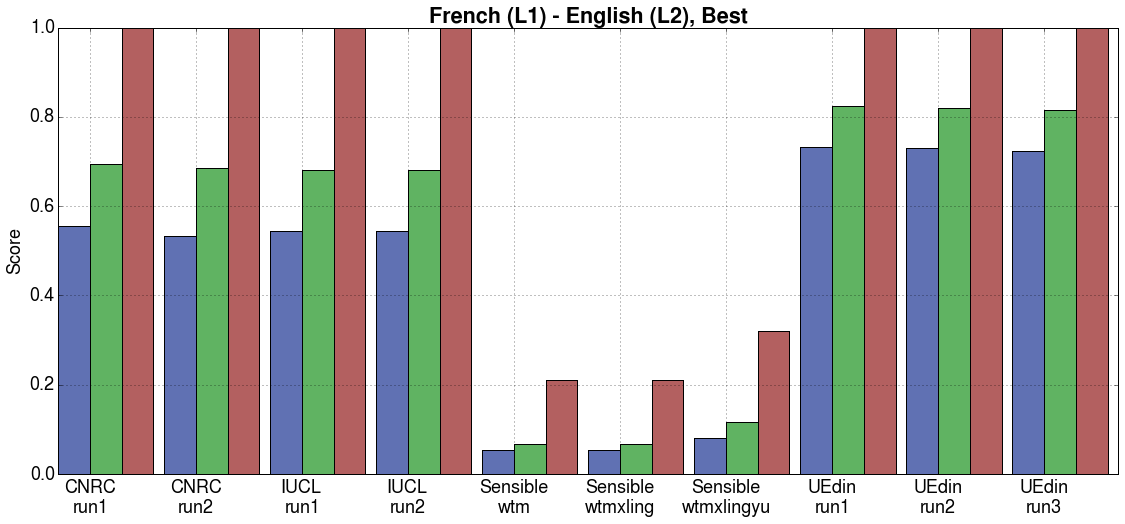
\includegraphics[width=16cm]{fr-en-best-2.png}}
\caption{English to Spanish (top), English to German (middle) and French to English (bottom). The three bars, left-to-right, represent Accuracy (blue), Word Accuracy (green) and Recall (red).}
\label{fig:graphs}
\end{figure*}

\section{Discussion}

We did not specify any training data for the task. The advantage of this is
that participants were free to build a wider variety of systems from various
sources, rather than introducing a bias towards for instances statistical
systems. The disadvantage, however, is that a comparison of the various systems
does not yield conclusive results regarding the merit of their methodologies.
Discrepancies might at least be partly due to differences in training data, as
it is generally well understood in MT that more training data improves results.
The baselines various participants describe in their system papers provide more
insight to the merit of their approaches than a comparison between them.

In the creation of the test set, we aimed to mimic intermediate to high-level
language learners. We also aimed at a fair distribution of different
part-of-speech categories and phrasal length. The difficulty of the task
differs between language pairs, though not intentionally so. We observe that
the Dutch-English set is the hardest and the Spanish-English is the easiest in
the task. One of the participants implicitly observes this through measurement
of the number of Out-of-Vocabulary words \citep{CNRC}. This implies that when
comparing system performance between different language pairs, one can not
simply ascribe a lower result to a system having more difficulty with said
language pair. This could rather be an intrinsic property of the test set or
the distance between the languages.

Distance in syntactic structure between languages also defines the limits of
this task. During composition of the test set it became clear that backing off
to L1 was not always possible when syntax diverged to much. An example of this
is separable verbs in Dutch and German. Consider the German sentence \emph{``Er
\textbf{ruft} seine Mutter \textbf{an}''} (translation: \emph{``He
\textbf{calls} his mother''}). Imagine a German language learner wanting to
compose such a sentence but wanting to fall back to English for the verb
\emph{``to call''}, which would translate to German as \emph{``anrufen''}. The
possible input sentence may still be easy to construe: \emph{``Er
\textbf{calls} seine Mutter''}, but the solution to this problem would require
insertion at two different points, whereas the task currently only deals with a
substitution of a single fragment. The reverse is arguably even more complex
and may stray too far from what a language learner may do. Consider an English
language learner wanting to fall back to her native German, struggling with the
English translation for \emph{``anrufen''}. She may compose a sentence such as
\emph{``He \textbf{ruft} his mother \textbf{an}''}, which would require
translating two dependent fragments into one.

We already have interesting examples in the gold standard, such as example (b),
showing syntactic word-order changes confined to a single fragment.

\begin{examples}
\footnotesize
%iris voorbeeld waar en-nl woordvolgende wisselt
\item[(b)] \textbf{Input:} I always wanted \textbf{iemand te zijn} , but now I realize I should have been more specific.\\
\textbf{Reference:} I always wanted \textbf{to be somebody} , but now I realize I should have been more specific.\\
\textbf{Participant output (aggregated):} to be a person; it to be; someone to his; to be somebody; person to be; someone to; someone to be; to be anybody; to anyone; to be someone; a person to have any; to be someone else
\end{examples}

Another question we can ask, but have not investigated, is whether a language
learner would insert the proper morphosyntactic form of an L1 word given the L2
context, or whether she may be inclined to fall back to a normal form such as
an infinitive. Especially in the above case of separable verbs someone may be
more inclined to circumvent the double fragments and provide the input:
\emph{``He \textbf{anrufen} his mother``}, but in simpler cases the same issue
arises as well. Consider an English learner falling back to her native
Croatian, a Slavic language which heavily declines nouns. If she did not know
the English word \emph{``book''} and wanted to write \emph{``He gave the book
to him''}, she could use either the Croatian word \emph{``knjigu''} in its
accusative declension or fall back to the normal form \emph{``knjiga''}. A
proper writing assistant system would have to account for both options.

We can analyse which of the sentences in the test data participants struggled
with most. First we look at the number of sentences that produce an average
word accuracy of zero, measured per sentence over all systems and runs in the
out-of-five metric. This means no participant was close to the correct output.
There were 6 such sentences in English-Spanish, 17 in English-German, 6 in
French-English, and 32 in Dutch-English.

%discuss user errors:
A particularly difficult context from the Spanish set is when a subjunctive
verb form was required, but an indicative verb form was submitted by the
systems, such as in the sentence: \emph{``Espero que los frenos del coche
\textbf{funcionen} bien.''}. Though this may be deduced from context (the word
\emph{``Espero''}, expressing hope yet doubt, being key here), it is often
subtle and hard to capture. Another problematic case that recurs in the German
and Dutch data sets is compound nouns. The English fragment \emph{``work
motivation''} should translate into the German compound
\emph{``Arbeitsmotivation''} or \emph{``Arbeitsmoral''}, yet participants were
not able to find the actual compound noun. Beside compound nouns, other less
frequent multi-word expressions are also amongst the difficult cases. Sparsity
or complete absence in training data of these expressions is why systems
struggle here.


%iris ik vind deze gewoon mooi:
%\textbf{Input:} Miami Beach is where neon {\emph naartoe gaat om te sterven }.\\
%\textbf{Reference:} Miami Beach is where neon \emph{ goes to die} .\\
%\textbf{Different participant output:} goes to die; is going to die; is going to go to die; goes of death; is going of death; go to die; are going to die; is being sent to of death; are allocated is of death; is heading of death; going to die; 's going to lead to die\\


Another point of discussion is the fact that we enriched the test set by adding
previously unavailable alternative translations from an aggregated pool of
system output. This might draw criticism for possibly introducing a bias, also
considering the fact that the decision to include a particular alternative for
a given context is not always straightforward and at times subjective. We,
however, contend that this is the best way to ensure that valid system output
is not discarded and reduce the number of false negatives. The effect of this
measure has been an increase in (word) accuracy for all systems, without
significant impact on ranking.


\begin{figure*}[bth] %cheating to get the figure at the same page
\noindent\makebox[\textwidth][c]{%
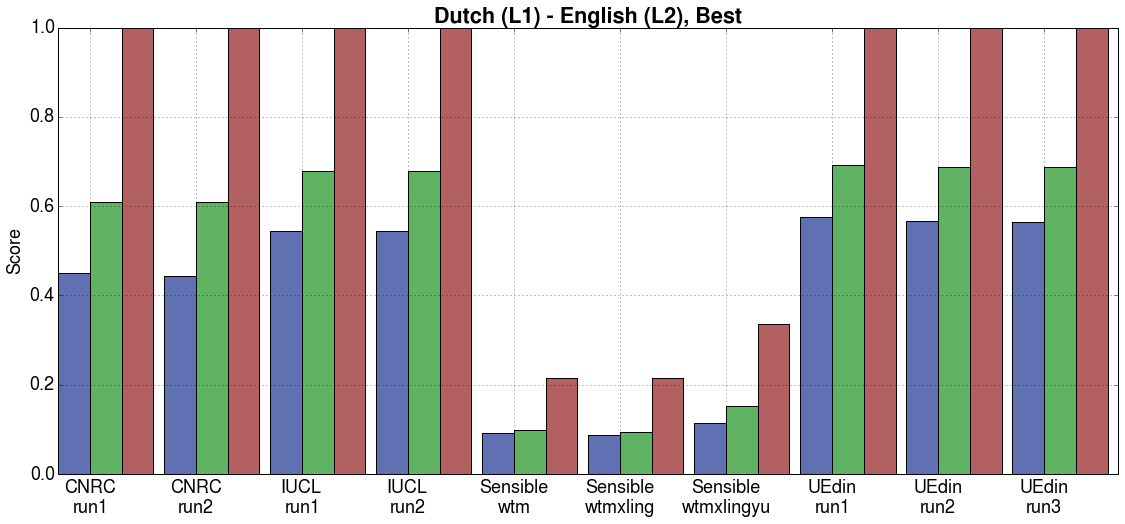
\includegraphics[width=16cm]{nl-en-best-2.png}
}
\caption{Dutch to English.}
\label{fig:graphs2}
\end{figure*}

\section{Conclusion}

In this SemEval task we showed that systems can translate L1 fragments in an L2
context, a task that finds application in computer-assisted translation and
computer-assisted language learning. The localised translation of a fragment in
a cross-lingual context makes it a novel task in the field. Though the task has
its limits, we argue for its practical application in a language-learning
setting: as a writing assistant and dictionary replacement. Six contestants
participated in the task, and used an ensemble of techniques from Statistical
Machine Translation and Word Sense Disambiguation. Most of the task organizers'
time went into manually establishing a gold standard based on a wide variety of
sources, most aimed at language learners, for each of the four language pairs
in the task. We have been positively surprised by the good results of the
highest ranking systems.

\section{Acknowledgements}

We would like to thank Andreu van Hooft and Sarah Schulz for their manual
correction work, and Sean Banville, Geert Joris, Bernard De Clerck, Rogier
Crijns, Adriane Boyd, Detmar Meurers, Guillermo Sanz Gallego and Nils Smeuninx
for helping us with the data collection.
